\documentclass[10pt]{beamer}
\usetheme{Berlin}
\usecolortheme{lily}
\usepackage[utf8x]{inputenc}
\usepackage[english]{babel}
\usepackage[T1]{fontenc}
\usepackage{lmodern}
\usepackage{amsmath}
\usepackage{amssymb}
\usepackage{enumerate}
\usepackage{graphicx}
\usepackage{cite}
\usepackage{listings}
\usepackage{hyperref}
\usepackage{lipsum}
\usepackage{tikz}
\beamertemplatenavigationsymbolsempty

\newcommand{\docauthor}{Axel Angel}
\newcommand{\doctitle}{Properties of CNN}
\newcommand{\docsubtitle}{Midterm Presentation}
\newcommand{\eg}{e.g.}
\newcommand{\reff}[1]{~\ref{#1}}
\setkeys{Gin}{width=1.0\textwidth}

\author{\docauthor}
\title{\docsubtitle}

\pdfinfo{
    /Author (\docauthor)
    /Title (\doctitle)
    /Subject (\docsubtitle)
    }

\begin{document}
\section{\doctitle}

% main subject (properties of cnn), don't use technical terms, why this happens 
\begin{frame}
    \frametitle{Motivations}
    \begin{itemize}
        \item What? Analysis of Convolutional Neutral Networks (CNNs)
        \item Why? Lab needs and personal interests
        \item How? Tools and experiments
    \end{itemize}
\end{frame}

% dataset (mnist), why present it before model, explain task (digits) and why (simple), stroke, why we choose this in our project (simple: no variance, we can play with)
\begin{frame}
    \frametitle{Dataset (\eg: MNIST)}
    \begin{itemize}
        \item Classical classification problem
        \item Popular and heavily ``normalized''
        \item Variance: digit, style, rotation, stroke thickness
        \item Invariance: uniform contrast, no background, upright, centered
        \item Why? High invariance (can artificially add them ourself)
    \end{itemize}

    \begin{figure}[h]
        \begin{center}
            
\includegraphics{midpres_figures/mnist.png}
        \end{center}
        \caption{Training samples}
    \end{figure}
\end{frame}

% what are cnn (layers, fwd/bwd, sgd, compare to other model: cnn learn own feature extraction, whereas svm/lr by hand)
\begin{frame}
    \frametitle{Short recap of CNNs}
    \begin{itemize}
        \item Architecture (layers, forward/backward SGD)
        \item LeNet (good, simple, popular choice), 0.7\% error
        \item Compare other models for MNIST (feature extraction)
    \end{itemize}

    \begin{figure}[h]
        \begin{center}
            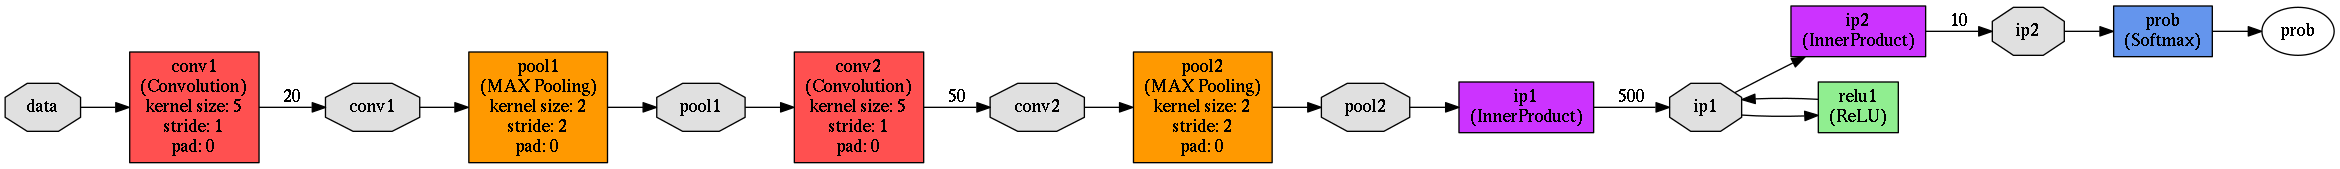
\includegraphics{midpres_figures/lenet.png}
        \end{center}
        \caption{LeNet architecture}
    \end{figure}
    \begin{figure}[h]
        \begin{center}
            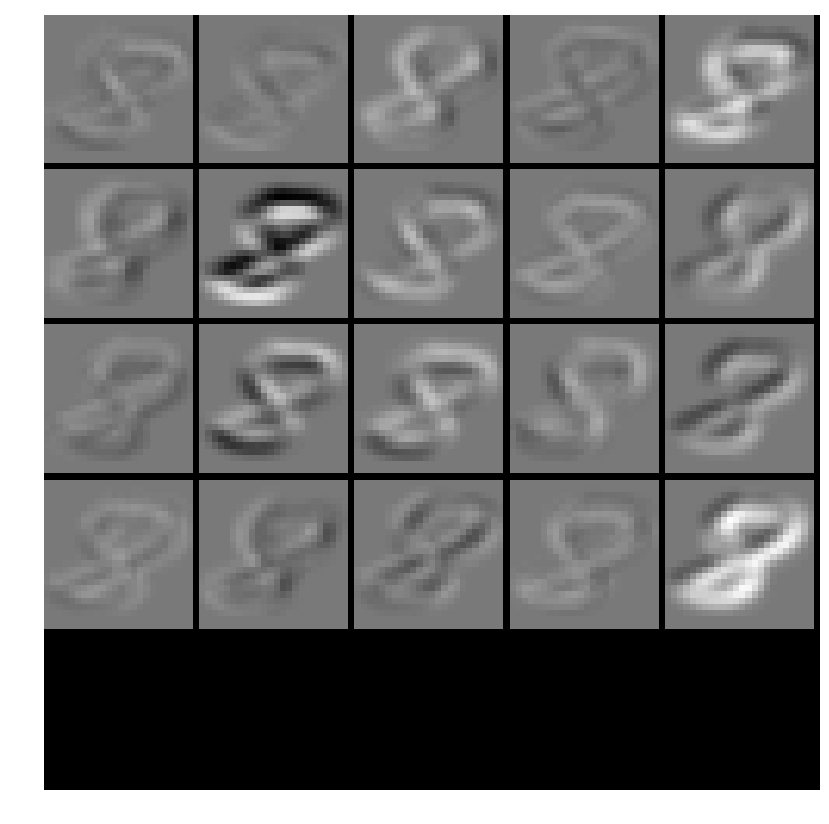
\includegraphics[width=0.45\textwidth]{midpres_figures/lenet_filter8.png}
        \end{center}
        \caption{LeNet features example}
    \end{figure}
\end{frame}

% previous works: cnn not well understood yet, intriguing properties (eg, adversials: classifier-recognizable vs human-recognizable), papers measure neuron activitation relation to patterns/translate/rotate
\begin{frame}
    \frametitle{Previous works}
    \begin{itemize}
        \item CNNs are not well understood yet
        \item Adversial noise and artificial images
        \item Relation between units/layers and features/deformations
        \item \dots and much more (but few gave insights)
    \end{itemize}
    \begin{figure}[h]
        \begin{tabular}[]{cc}
            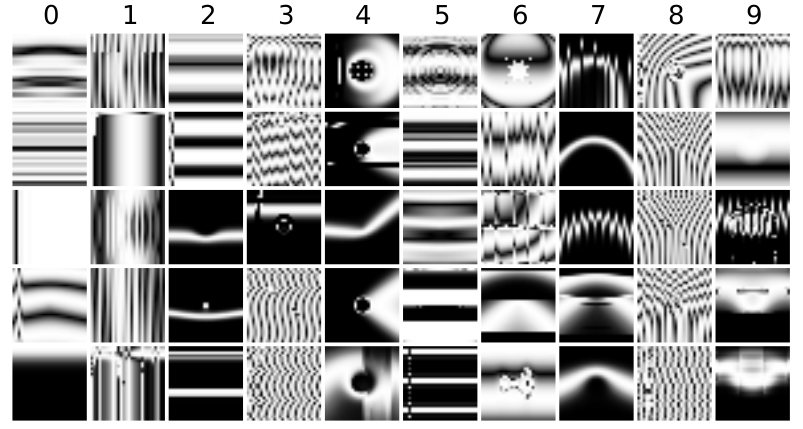
\includegraphics[width=0.45\textwidth]{midpres_figures/adversial_unrecogni.png}
            &
            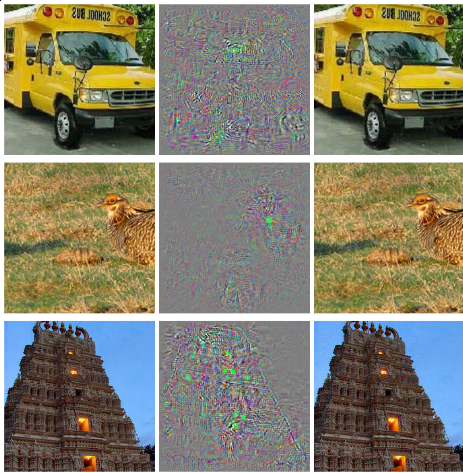
\includegraphics[width=0.3\textwidth]{midpres_figures/adversial_imagenet.png}
        \end{tabular}
        \caption{Adversial images}
    \end{figure}
\end{frame}

% our researches: vector space analysis (t-sne=tool), invariance analysis then training using data augmentation (transformations: attacks by adversial, translate/rotate data-augmentation); they are related, complementary
\begin{frame}
    \frametitle{Our work}
    Two complementary axises:
    \begin{itemize}
        \item Invariance analysis (data-augmentation and adversial attacks)
        \item Vector-space analysis (\eg: t-SNE)
    \end{itemize}
\end{frame}

% findings on data-augmentation training (why, results, conclusions)
\begin{frame}
    \frametitle{Data-augmentation training}
    Image transformations: for training
    \begin{itemize}
        \item Data-augmentation
        \item Invariance Training (particular case)
        \item Why?
        \item Experiments and results
            % feh test*-v3{a,b}.png
        \item Conclusions
    \end{itemize}
\end{frame}

% findings on t-sne applied to mnist (explain vector space, why t-sne? visualize, high dims space, keep closeness), (1) regular model without data-augmentation model (2) with shift-invariance -> crowded; model distinguish translation first (big clusters) then subclusters = digit
\begin{frame}
    \frametitle{Vector-space analysis}
    \begin{itemize}
        \item Visualization: t-SNE\footnote{t-Distributed Stochastic Neighbor Embedding (t=student distribution)} (2D map preserving closeness)
        \item Optimisation problem: Model pair-distance by student-distribution, find a good equivalent distribution in 2D (Kullback-Leibler divergence).
        \item Visually inspect high-dim vector-space using t-SNE: transformations and training
        % data_mnist/save_t-sne_transfo-v5-orig_10k_ip1_i0-9a-e_1427464401.js
        % data_mnist/save_t-sne_transfo-v4-shift4_10k_ip1_i0-9a-e_1427450541.js
    \end{itemize}
\end{frame}

% findings on adversial attacks (some examples and accuracies)
\begin{frame}
    \frametitle{Adversial attacks\footnote{WARNING: early results}}
    Image transformations: for attacks
    \begin{itemize}
        \item Adversial generation
        \item Examples
            % feh midpres_figures/adv1{_scaled,}*.png
            % (early results: feh test_transfo_adversial_correct.png )
    \end{itemize}
\end{frame}


%  next steps:
% * analysis of adversial attack (better graphs, data-augmented adversial training)
% * compare distance between original image and adversial in image space versus vector space (in which layer it happens), write code to detect the responsible weights for divergence (for adversial) or convergence (for invariance), comparing two models
\begin{frame}
    \frametitle{Next steps}
    \begin{itemize}
        \item Analysis of adversial attacks
        \item Tools to correlate neurons and distances between image-vector spaces
        \item Understand neurons responsibility: for adversials, for invariance
        \item Generalize to other datasets (\eg: BSDS, ImageNet)
    \end{itemize}
\end{frame}

\end{document}
